% Page: Reliability
% sources/stat2003/chapters/prob-07-reliability.qmd
% Hazard h(t)=lambda*beta*(lambda*t)^{beta-1}. Shape beta=1 is the exponential
% law, a constant hazard. beta>1 ages; beta<1 becomes less prone to failure.
% Drawn at lambda=1, so h(t)=beta*t^{beta-1}.
\documentclass[border=6pt]{standalone}
\usepackage[T1]{fontenc}
\usepackage{lmodern}
\usepackage{amsmath,amssymb}
\usepackage{tikz}
\usepackage{pgfplots}
\pgfplotsset{compat=1.18}
\definecolor{ink}{HTML}{1F2430}
\definecolor{statblue}{HTML}{174A7E}
\definecolor{accent}{HTML}{9C4A32}
\definecolor{grey}{HTML}{5E6A75}
\pgfplotsset{
  stat/.style={
    scale only axis,
    axis lines=left,
    axis line style={ink, line width=0.6pt},
    tick style={ink, line width=0.45pt},
    tick label style={font=\small, text=ink},
    label style={font=\small, text=ink},
    title style={font=\small, text=ink, align=center},
    legend style={font=\small, draw=none, fill=none, text=ink,
      cells={anchor=west}, inner sep=1.5pt,
      at={(0.50,0.98)}, anchor=north},
    unbounded coords=jump,
    scaled ticks=false,
    every axis plot/.append style={line width=0.9pt, line join=round},
  },
}
\begin{document}
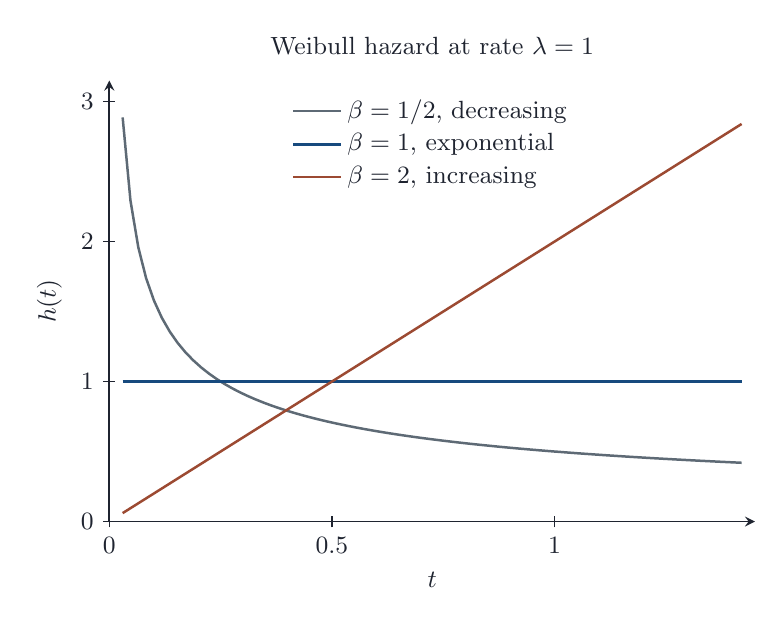
\begin{tikzpicture}
\begin{axis}[
  stat, width=8.2cm, height=5.6cm,
  xmin=0, xmax=1.45, ymin=0, ymax=3.15,
  xtick={0,0.5,1},
  ytick={0,1,2,3},
  xlabel={$t$},
  ylabel={$h(t)$},
  title={Weibull hazard at rate $\lambda=1$},
  domain=0.03:1.42, samples=80,
]
  \addplot[grey] {0.5*x^(-0.5)};
  \addlegendentry{$\beta=1/2$, decreasing}
  \addplot[statblue] {1};
  \addlegendentry{$\beta=1$, exponential}
  \addplot[accent] {2*x};
  \addlegendentry{$\beta=2$, increasing}
\end{axis}
\end{tikzpicture}
\end{document}
